\documentclass[10.5pt,notitlepage]{article}
\usepackage[utf8]{inputenc}
\usepackage{amsthm}
\usepackage{amsmath}
\usepackage{amsfonts}
\usepackage{mathtools}
\usepackage{amsmath,amssymb}       
\usepackage{enumitem}   
\usepackage{enumerate}
\usepackage{bbm}
\usepackage{booktabs}
\renewcommand{\qedsymbol}{$\blacksquare$}
\usepackage{makecell}
\usepackage[spanish]{babel}
\decimalpoint
\usepackage[letterpaper]{geometry}
\usepackage{mathrsfs}
\newenvironment{solucion}
  {\begin{proof}[Solución]}
  {\end{proof}}
\pagestyle{plain}
\usepackage{pdflscape}
\usepackage[table, dvipsnames]{xcolor}
\usepackage{longtable}
\usepackage{tikz}
\def\checkmark{\tikz\fill[scale=0.4](0,.35) -- (.25,0) -- (1,.7) -- (.25,.15) -- cycle;} 
\usepackage[bottom]{footmisc}
\usepackage{hyperref}
\usepackage{float}
\usepackage[utf8]{inputenc}
\usepackage{bbm}
\usepackage{placeins}
\newcommand{\pp}{\mathbb{P}}
\newcommand{\BB}{\mathcal{B}}
\newcommand{\RR}{\mathbb{R}}
\newcommand{\FF}{\mathcal{F}}
\newcommand{\CC}{\mathcal{C}}
\newcommand{\oo}{\varnothing}
\newcommand{\ee}{\varepsilon}
\newcommand{\NN}{\mathbb{N}}
\newcommand{\PP}{\mathcal{P}}
\newcommand{\LL}{\mathrm{L}}
\newcommand{\XX}{\mathbf{X}}
\newcommand{\xx}{\mathcal{X}}
\newcommand{\abs}[1]{\left\lvert #1 \right\rvert}
\newcommand{\norm}[1]{\left\| #1 \right\|}
\newcommand{\inner}[1]{\left\langle #1 \right\rangle}
\newcommand{\corch}[1]{\left[ #1 \right]}
\newcommand{\kis}[1]{\left\{ #1 \right\}}
\newcommand{\pare}[1]{\left( #1 \right)}

\theoremstyle{plain}

\newtheorem{thm}{Teorema}[section] % reset theorem numbering for each chapter
\newtheorem{defn}[thm]{Definición} % definition numbers are dependent on theorem numbers
\newtheorem{lem}[thm]{Lema} % same for example numbers
\usepackage{geometry}
\usepackage{mathtools}
\usepackage{enumitem}
\usepackage{framed}
\usepackage{amsthm}
\usepackage{thmtools}
\usepackage{etoolbox}
\usepackage{fancybox}

\newenvironment{myleftbar}{%
\def\FrameCommand{\hspace{0.6em}\vrule width 2pt\hspace{0.6em}}%
\MakeFramed{\advance\hsize-\width \FrameRestore}}%
{\endMakeFramed}
\declaretheoremstyle[
spaceabove=6pt,
spacebelow=6pt
headfont=\normalfont\bfseries,
headpunct={} ,
headformat={\cornersize*{2pt}\ovalbox{\NAME~\NUMBER\ifstrequal{\NOTE}{}{\relax}{\NOTE}:}},
bodyfont=\normalfont,
]{exobreak}

\declaretheorem[style=exobreak, name=Ejercicio,%
postheadhook=\leavevmode\myleftbar, %
prefoothook = \endmyleftbar]{exo}
\usepackage{graphicx}
\graphicspath{ {images/} }
\title{Tarea 4: Modelos Estadísticos I.}

\author{Rojas Gutiérrez Rodolfo Emmanuel}

\date{\today}

\begin{document}

\maketitle

\setcounter{exo}{0}
\begin{exo}
Los datos de la Figura \ref{fig:1} se han ordenado de manera conveniente para poder ver la relación 
entre la varianza de la respuesta y la variable explicativa. La muestra consta de 33 observaciones $(X_i,Y_i)$
con un número de conjuntos que tienen repeticiones exactas de la $X$ o repeticiones aproximadas. Estos 
conjuntos están indicados por las agrupaciones.
    \begin{itemize}
        \item[(a)] Ajuste un modelo de regresión lineal simple, por mínimos cuadrados no ponderados 
        \item[(b)] Haga una gráfica de residuos contra valores ajustados. Comente la gráfica. 
        \item[(c)] Haga una gráfica de residuos contra valores de la variable independiente. Comente la gráfica. 
        \item[(d)] ¿Qué relación tiene la varianza (de las 
         $Y_s$) con los valores de la variable explicativa? ¿Lineal, 
          cuadrática o cubica? 
        \item[(e)] Asigne los pesos $\hat{w}_i=\hat{\sigma}^{-2}$ que les corresponden a las observaciones (llenar la tercera columna de la 
         Tabla en la Figura \ref{fig:1}). 
        \item[(f)] Ajuste el modelo de regresión lineal simple por mínimos cuadrados ponderados. 
        \item[(g)] Compare y comente los ajustes de los incisos (a) y (f).
    \end{itemize}
\end{exo}
\begin{figure}[htb]
 \centering
 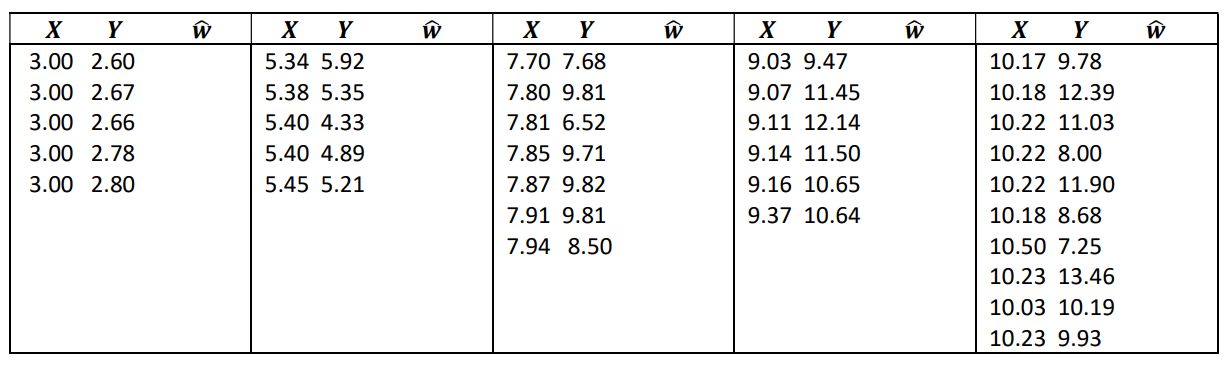
\includegraphics[scale=0.40]{T3T.png}
 \caption{Datos para el problema de mínimos cuadrados ponderados.}
 \label{fig:1}
\end{figure}
\begin{solucion}
\noindent \textbf{(a)} Se ajustará un modelo de regresión lineal simple a los datos presentados en la Figura \ref{fig:1}, en el que se consideraran términos de error \(i.i.d\) con media \(0\) y varianza constante \(\sigma^2 > 0\), es decir que 
\[
Y = \mathbf{X}\beta + \ee, 
\]
donde:
\begin{equation}\label{mod 1}
\beta = \begin{pmatrix}
\beta_0\\ 
\beta_1
\end{pmatrix}, \quad
    \mathbf{X} = 
      \bordermatrix{
 &\mathrm{1}&X\cr
& 1.0 &  3.0\cr
& 1.0 &  3.0\cr
& 1.0 &  3.0\cr
& 1.0 &  3.0\cr
& 1.0 &  3.0\cr
& 1.0 &  5.34\cr
& 1.0 &  5.38\cr
& 1.0 &  5.4\cr
& 1.0 &  5.4\cr
& 1.0 &  5.45\cr
& 1.0 &  7.7\cr
& 1.0 &  7.8\cr
&1.0 &  7.81\cr
&\vdots&\vdots\cr 
& 1.0 &  9.16\cr
& 1.0 &  9.37\cr
& 1.0 & 10.17\cr
& 1.0 & 10.18\cr
& 1.0 & 10.22\cr
& 1.0 & 10.22\cr
& 1.0 & 10.22\cr
& 1.0 & 10.18\cr
& 1.0 & 10.5\cr
& 1.0 & 10.23\cr
& 1.0 & 10.03\cr
& 1.0 & 10.23
  },\quad Y = \begin{pmatrix} 
 2.6\\
  2.67\\
  2.66\\
  2.78\\
  2.8\\
  5.92\\
  5.35\\
  4.33\\
  4.89\\
  5.21\\
  7.68\\
  9.81\\
  6.52\\
  \vdots\\
 10.65\\
 10.64\\
  9.78\\
 12.39\\
 11.03\\
  8.0\\
 11.9\\
  8.68\\
  7.25\\
 13.46\\
 10.19\\
  9.93
\end{pmatrix},
\end{equation}
y \(\ee\) es el vector de términos de error, a partir de este punto se hará referencia a la columna \(X\) de la matriz \(\textbf{X}\) como los valores de la variable independiente, o incluso se le denominará variable independiente. De este modo las estimaciones por mínimos cuadrados para \(\beta = \begin{pmatrix}
\beta_0\\ 
\beta_1
\end{pmatrix}\) están dados por:
\begin{equation}
   \hat{\beta} = \begin{pmatrix}
\hat{\beta}_0\\ 
\hat{\beta_1}
\end{pmatrix} = (\mathbf{X}^{'}\mathbf{X})^{-1}\mathbf{X}^{'}Y = \begin{pmatrix}
 -0.506\\ 
 1.127
\end{pmatrix}.
\end{equation}
Por lo que, la ecuación de regresión para la estimación de la media de la variable dependiente \(Y\) dado un valor de la variable independiente \(X\) esta dada por: 
\begin{equation}\label{ec1}
    \hat{E}[Y_i|X_i] = -0.506 + 1.127X_i, \ i\in\kis{1, \hdots, 33}. 
\end{equation}
Por otro lado, el coeficiente de determinación para este modelo esta dado por 
\begin{equation}\label{R^21}
    R_{OLS}^2 = \frac{\beta^{'}\mathbf{X}^{'}Y - n \overline{Y}^2}{Y^{'}Y - n \overline{Y}^2} =  0.796. 
\end{equation}
Para concluir este inciso se muestra en la Figura \ref{fig:3} una gráfica con los datos de la Figura \ref{fig:1}, la correspondiente recta de regresión lineal \eqref{ec1} y bandas de confianza y predicción al \(95\%\) de confianza. Esto con la finalidad de comparar está gráfica con el futuro modelo de mínimos cuadrados ponderados que se ajustará posteriormente. \\
\begin{figure}[htb]
 \centering
 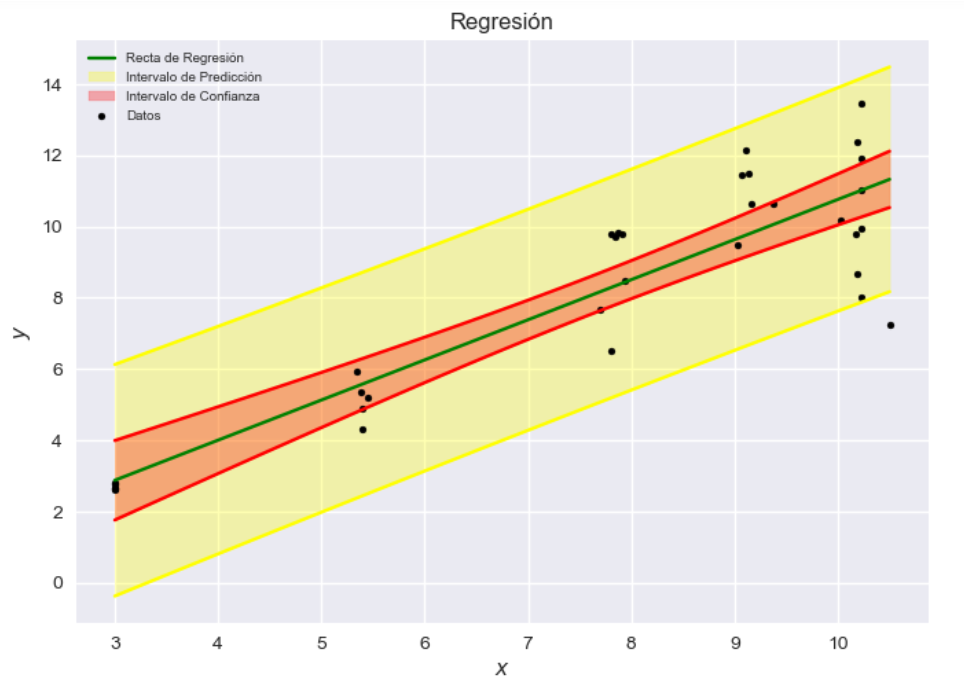
\includegraphics[scale=0.40]{OLS.png}
 \caption{Modelo de Regresión Lineal Simple Ajustado por MCO, con Bandas de Predicción y Confianza al \(95\%\).}
 \label{fig:3}
\end{figure}

\noindent \textbf{(b)} La gráfica solicitada se presenta en la Figura \ref{fig:4}, los datos se encuentran clasificados por colores uno por cada uno de los 5 grupos dados en un inicio, donde los grupos se han etiquetado como \(G_1,G_2,\hdots,G_5\) y representan a cada una de las 5 columnas de la tabla \ref{fig:1} respectivamente. Ahora, dado que los residuales y los valores ajustados son elementos aleatorios no correlacionados, si es que se cumplen los supuestos del modelo de regresión lineal simple, entonces no se debería de notar una relación entre dichas cantidades observadas y se esperaría que los residuales se vieran dispersos como variables aleatorias de media \(0\) y varianza constante\footnote{Pese a que no son de varianza constante, pero al ser las estimaciones de los errores deberían reflejar en cierto modo su comportamiento.}, sin embargo en la gráfica construida es fácil observar que conforme crece el valor ajustado \(\hat{Y}\) también lo hace la dispersión que existe entre los residuales. Como observación importante tome en cuenta que la varianza parece cambiar a través de los grupos.\\
\begin{figure}[htb]
 \centering
 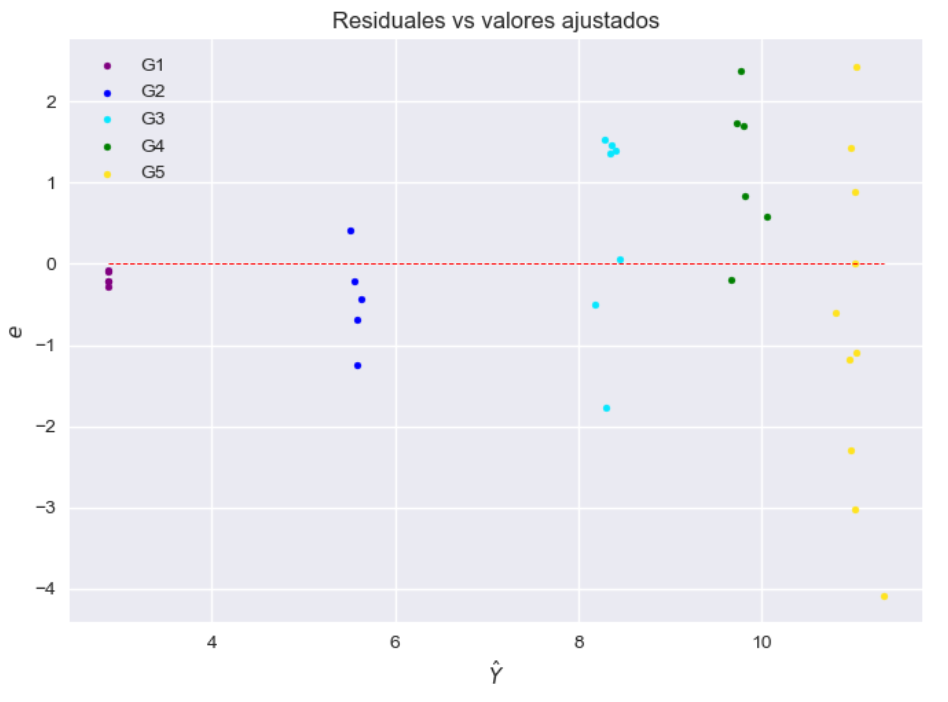
\includegraphics[scale=0.40]{Residuales vs Ajustes.png}
 \caption{Gráfica de residuales vs Valores Ajustados.}
 \label{fig:4}
\end{figure}

\noindent \textbf{(c)} La gráfica solicitada se presenta en la Figura \ref{fig:5}, nuevamente los datos se encuentran clasificados por colores de manera análoga a como se hizo en el inciso \textbf{(b)}. Dado que el valor de la variable independiente no debería influir en el comportamiento de los residuales, bajo los supuestos del modelo de regresión lineal simple, entonces la dispersión de los residuales a través de los diferentes valores de la variable independiente \((X)\) debería ser la misma, sin embargo se observa un patrón similar al que se tenía en la gráfica del inciso \textbf{(b)}, es decir conforme aumenta el valor de la variable independiente también parece incrementar la variabilidad de los residuales respecto al \(0\), este último hecho era de esperarse dado que \(\beta_1 X_i = \hat{Y_i}\) con \(\beta_1 = 1.127\), es decir los valores ajustados y los valores de la variable independiente están relacionados linealmente mediante un coeficiente de pendiente positivo. De este modo, los incisos \textbf{(b)} y \textbf{(c)} parecen indicar la existencia de cierta heterocedasticidad en la variabilidad de los errores\footnote{finalmente igual a la variabilidad de las observaciones.}, relacionada con la variable independiente \(X\), por lo que un modelo de regresión lineal simple ajustado por mínimos cuadrados ponderados podría ser mas sensato para estos datos, que uno de regresión lineal simple ajustado por MCO.

\begin{figure}[htb]
 \centering
 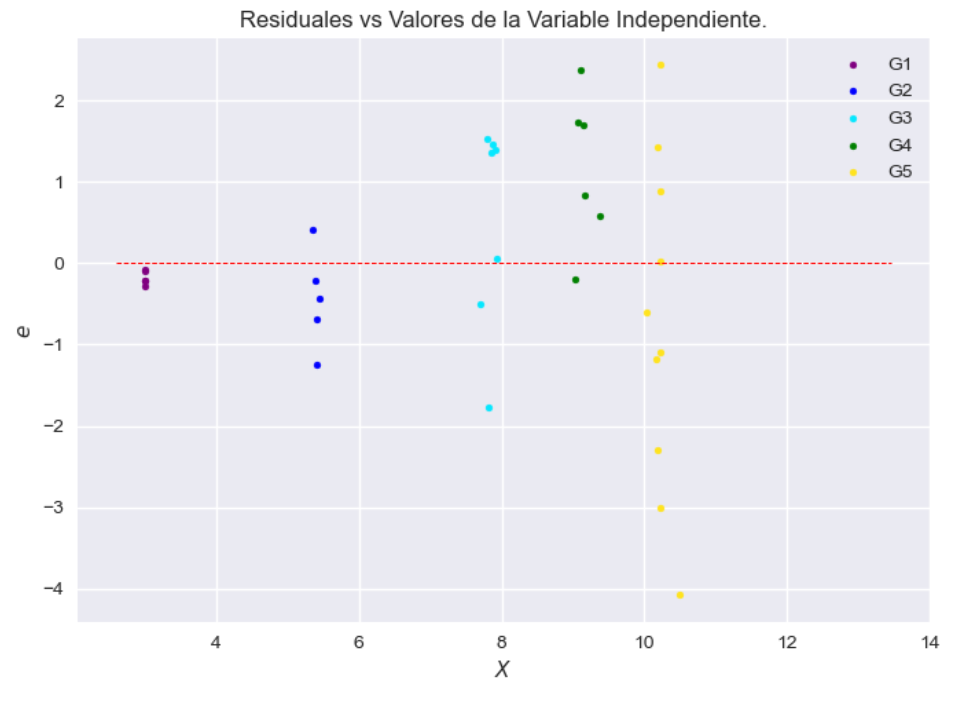
\includegraphics[scale=0.40]{Residuales vs VI.png}
 \caption{Gráfica de residuales vs Valores de la Variable Independiente.}
 \label{fig:5}
\end{figure}

\noindent \textbf{(d)} Dado que se esta pensando en ajustar un modelo por mínimos cuadrados ponderados, y dado que pareciera que el valor de la variable independiente afecta de manera directa a la variabilidad de las observaciones, este inciso tendrá como finalidad encontrar de que manera es que se da esta dependencia, ya que la misma ayudará a establecer los pesos adecuados para el ajuste del modelo. Para ello se realizó el siguiente análisis, se obtuvo la varianza muestral de las observaciones para cada uno de los 5 grupos,\footnote{Sí se ha pecado de obviedad, por ejemplo se tendrá que la primer varianza corresponde a la varianza muestral de los valores de \(Y\), en la primera sección de la Tabla en la Figura \ref{fig:1} y por ende las primeras \(5\) entradas de \(\sigma^2\) corresponderán a este valor, luego se pasa la segunda sección de la tabla y se repite el procedimiento.} dichos valores se representaran de manera vectorial como \(\sigma^2\) y a las componentes de este vector como \(\sigma_i^2\), con estos datos se realizó una gráfica de los valores de la variable independiente \((X)\) contra la varianza muestral de las observaciones de la variable dependiente \((Y)\) por grupo, dando como resultado el gráfico mostrado en la Figura \ref{fig:6}.\footnote{Los grupos nuevamente se destacaron por colores de manera análoga a como se hizo en los incisos \textbf{(b)} y \textbf{(c)}.}
\begin{figure}[htb]
 \centering
 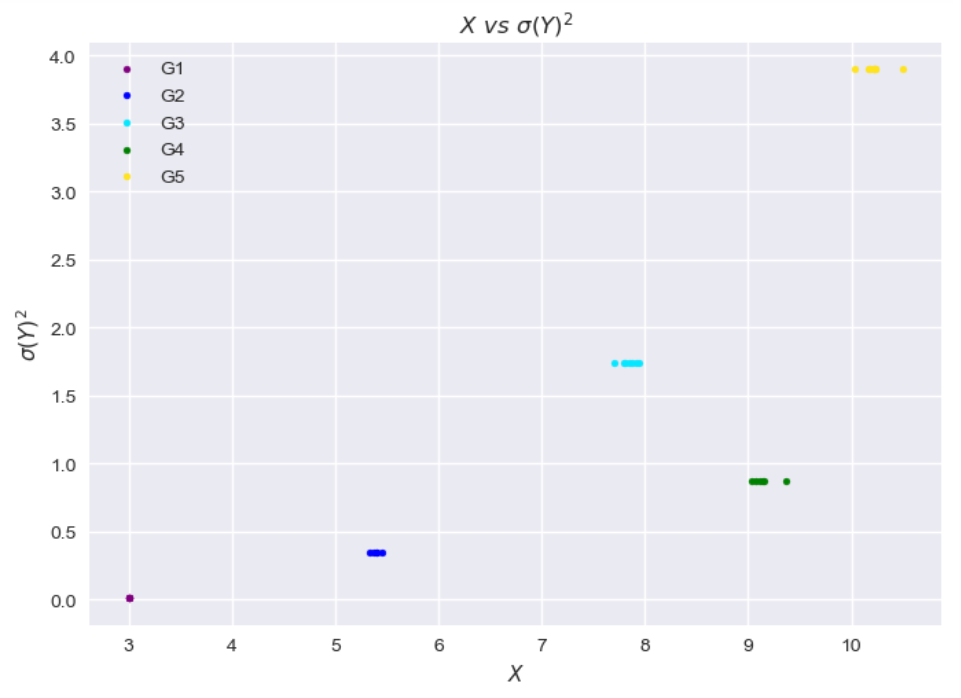
\includegraphics[scale=0.40]{medias.png}
 \caption{Gráfica Variable Independiente vs Varianzas por Grupo.}
 \label{fig:6}
\end{figure}\\
Utilizando los datos anteriores se ajustaron:
\begin{enumerate}
    \item Un polinomio lineal: \(a_0 + a_1 x\).
    \item Un polinomio cuadrático: \(b_0 + b_1 x + b_2 x^2\), 
    \item Un polinomio cúbico: \(c_0 + c_1 x + c_2 x^2 + c_3 x^3\).
\end{enumerate}
Los ajustes se realizaron por Mínimos Cuadrados Ordinarios (MCO), utilizando como variable explicativa los valores de la variable independiente\footnote{Independiente respecto al modelo original.} y como variable explicada a los valores de las varianzas muéstrales de la variable dependiente por grupo, obteniendo los siguientes resultados
\begin{align}\label{Ajus1}
     \sigma_i^{2} &= -1.973 + 0.485 X_i, \ i \in \kis{1, \hdots, 33}, \quad R^2 = 0.663,\nonumber \\ 
     \sigma_i^{2} &=  1.808 -0.847X_i + 0.098X_i^{2}, \ i\in\kis{1, \hdots, 33}, \quad R^2 =0.776,\nonumber \\ 
     \sigma_i^{2} &= -6.235+ 3.588X_i -0.617X_i^{2} + 0.035X_{i}^{2}, \ i\in\kis{1, \hdots, 33}, \quad R^2 =0.825, 
\end{align}
Al ajustar estos tres polinomios se identificaron dos problemas. El primero es que el coeficiente \(R^2\) siempre se vuelve más grande cuando se introduce una covariable extra, por ende si se ajustará un modelo de grado cuarto su coeficiente de determinación sería aún mayor que el de los modelos en \eqref{Ajus1}, sin embargo ese incremento no premiaría la parsimonia del modelo. Por otra parte, es fácil observar en la gráfica presentada en la Figura \ref{fig:7}, que los valores que se generarían con este ajuste tendrían posibilidad de ser negativos en el intervalo formado por el mínimo de las observaciones de \(X\) y el máximo de las mismas, lo cual no es deseable debido a que se esta modelando la varianza de la variable dependiente, que como se sabe es una cantidad no negativa.  
\begin{figure}[htb]
 \centering
 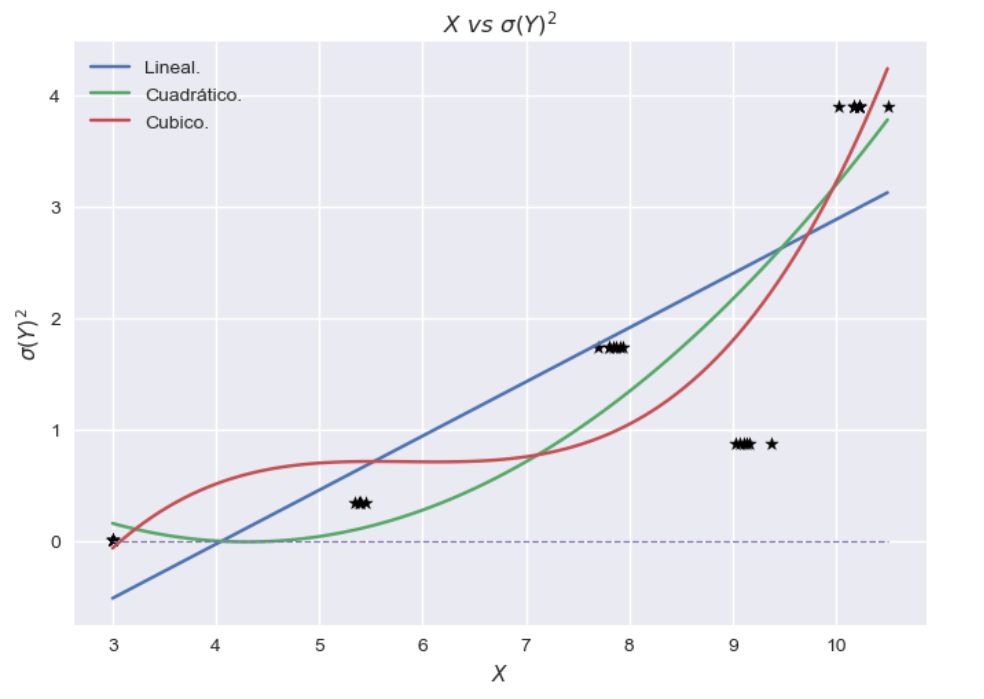
\includegraphics[scale=0.40]{ajustes polinomicos1.png}
 \caption{Gráfica Polinomios Ajustados Por MCO I.}
 \label{fig:7}
\end{figure}\\ 

A modo de confirmación de este hecho, es posible verificar en el script adjunto a esta tarea que efectivamente el mínimo de cualquiera de estos polinomios en el intervalo mencionado es menor a cero. Para evitar estos problemas, se decidió intentar ajustar alguna de las siguientes dos opciones\footnote{Observe que dada la relación creciente que existe entre \(X\) y \(\sigma^2\), se esperaría que las estimaciones de los coeficientes \(b_2\) y \(c_3\) fueran no negativas, lo que evitaría el problema de los pesos negativos.}:
\begin{enumerate}
    \item Un polinomio cuadrático: \(b_2 x^2\), 
    \item Un polinomio cúbico: \(c_3 x^3\),
\end{enumerate}
El modelo lineal se descartó por completo, debido al pobre desempeño mostrado en la Figura \ref{fig:7}. Los ajustes nuevamente se realizaron ocupando la técnica de MCO obteniendo los siguientes resultados: 
\begin{align}\label{Ajus2}
     \sigma_i^{2} &=  0.0291X_i^{2}, \ i\in\kis{1, \hdots, 33}, \quad R^2 =0.867,\nonumber \\ 
     \sigma_i^{2} &=  0.0031X_{i}^{3}, \ i\in\kis{1, \hdots, 33}, \quad R^2 =0.9002,
\end{align}
pudiera sorprender al lector que el coeficiente de determinación en los modelos \eqref{Ajus2}, sea mayor que el de los modelos en \eqref{Ajus1} dado el comentario de que el agregar covariables siempre incremente su valor, pero dado que los modelos propuestos se han tomado sin intercepto es necesario hacer una modificación al calculo del coeficiente de determinación,\footnote{Dicha modificación se explicará en el anexó a este trabajo.} la cual además premia la parsimonia de los modelos anteriores. Tomando entonces en cuenta los coeficientes de determinación de los modelos en \eqref{Ajus2}, se concluye para efectos de este inciso que la relación existente entre la varianza de las observaciones y la variable independiente \(X\) es cúbica de la forma
\begin{equation}\label{Var}
     \sigma_i^{2} = \sigma^2 \cdot X_{i}^{3}, \ \sigma^2 >0, \ i\in\kis{1, \hdots, 33}
\end{equation}.

\noindent \textbf{(e)} Sean \(\mathbf{X},Y\) y \(\beta\) como en \eqref{mod 1} se intentará ajustar un modelo de regresión lineal simple por Mínimos Cuadrados Ponderados (MCP), es decir se intentará estimar el vector de parámetros \(\beta\) para 
\begin{equation}\label{model2}
    Y = \mathbf{X} \beta + \ee, 
\end{equation}
pero a diferencia del inciso \textbf{(a)} se trabajará bajo el supuesto de que \(\ee\) es un vector de términos de error, tales que \(E(\ee) = 0 \) y \(V(\ee) = \sigma^2 V\) donde \(V\) se tomará por \eqref{Var} de la siguiente forma:\footnote{Esto quiere decir que se mantiene el supuesto de de independencia entre los términos de error, más no el supuesto de varianza constante entre los mismos. Por otro lado, observe que una estimación de \(\sigma_1^{2}\) esta dada por \eqref{Ajus2} y es igual a \(0.0031\).} 
\begin{equation}\label{VV}
V =\begin{pmatrix}
       X_{1}^{3} & 0      & \vdots  & 0 &0 \\ 
      0 &  X_{2}^{3}   & \vdots  & 0 &0 \\ 
      \hdots & \hdots & \ddots  & \hdots &\hdots \\ 
      0 & 0           & \vdots  &    X_{32}^{3} &0 \\ 
      0 & 0           & \vdots  & 0 &  X_{33}^{3}
\end{pmatrix}.
\end{equation}
De este modo, los pesos \(\omega_i\) quedan dados por los valores en la diagonal de la inversa de la matriz \(V\), dado que esta última es una matriz diagonal bastará con tomar la matriz diagonal cuyas entradas corresponden a los recíprocos de las entradas en la diagonal de \(V\), esto es posible debido a que los 33 valores de la columna \(X\) de la matriz \(\mathbf{X}\) son positivos, de este modo 
\begin{equation}
    V^{-1} =\begin{pmatrix}
      X_{1}^{-3} & 0      & \vdots  & 0 &0 \\ 
      0 &  X_{2}^{-3}   & \vdots  & 0 &0 \\ 
      \hdots & \hdots & \ddots  & \hdots &\hdots \\ 
      0 & 0           & \vdots  &    X_{32}^{-3} &0 \\ 
      0 & 0           & \vdots  & 0 &  X_{33}^{-3} 
\end{pmatrix}.
\end{equation}
Así pues, la Tabla en la Figura \ref{fig:1} se completa utilizando que \(\omega_i = X_{i}^{-3}\) es el peso asociado a la varianza de \(Y_i\), con \(i = 1, \hdots, 33\), de la manera que se presenta en los Cuadros \ref{tab:1} y \ref{tab:2}.  
\begin{table}[htb]
\centering
\scalebox{0.9}{
\begin{tabular}{@{}|rrr|rrr|rrr|@{}}
\toprule
\(X\)&\(Y\)&\(\omega\) &\(X\)&\(Y\)&\(\omega\) &\(X\)&\(Y\)&\(\omega\) \\
 \midrule
3.00&2.60 &3.704\cdot10^{-2} &5.34 &5.92 &6.567\cdot10^{-3} &7.70 &7.68 &2.190\cdot10^{-3} \\  
3.00&2.67 &3.704\cdot10^{-2} &5.38 &5.35 &6.422\cdot10^{-3} &7.80 &9.81 &2.107\cdot10^{-3} \\  
3.00&2.66 &3.704\cdot10^{-2}&5.40 &4.33 &6.351\cdot10^{-3} &7.81 &6.52 &2.099\cdot10^{-3}  \\  
3.00&2.78 &3.704\cdot10^{-2}&5.40 &4.89 &6.351\cdot10^{-3} &7.85 &9.71 &2.067\cdot10^{-3} \\  
3.00&2.80 &3.704\cdot10^{-2}&5.45 &5.21 &6.177\cdot10^{-3} &7.87 &9.82 &2.052\cdot10^{-3}  \\  
 & &                        &     &     &                  &7.91&9.81  &2.021\cdot10^{-3}  \\  
 & &                        &     &     &                  &7.94 &8.50  &1.998\cdot10^{-3}  \\  
 & &                        &     &     &                  &     &      &                 \\  
 & &                        &     &     &                  &     &      &                  \\ 
 & &                        &     &     &                  &     &      &               \\
\bottomrule
\end{tabular} 
}

\caption{Tabla de Datos con Ponderadores (Redondeados a 3 Dígitos Después del Punto Decimal).}
\label{tab:1}
\end{table}
\begin{table}[htb]
\centering
\scalebox{0.9}{
\begin{tabular}{@{}|rrr|rrr|@{}}
\toprule
\(X\)&\(Y\)&\(\omega\) &\(X\)&\(Y\)&\(\omega\) \\
\midrule
 9.03 &9.47  &1.358\cdot10^{-3}  &10.17 &9.78 & 9.507\cdot10^{-4}\\
 9.07 &11.45 & 1.340\cdot10^{-3} & 10.18 &12.39& 9.479\cdot10^{-4}\\
 9.11 &12.14 & 1.323\cdot10^{-3} &10.22 &11.03 & 9.368\cdot10^{-4}\\ 
 9.14 &11.50 & 1.310\cdot10^{-3} &10.22 &8.00 & 9.368\cdot10^{-4}\\ 
 9.16 &10.65 &1.301\cdot10^{-3}  &10.22 &11.90 & 9.368\cdot10^{-4}\\  
 9.37 &10.64 &1.216\cdot10^{-3}&10.18 &8.68 & 9.479\cdot10^{-4}\\
     &       &  &10.50 &7.25 & 8.638\cdot10^{-4}\\ 
     &       &  &10.23 &13.46 &9.341\cdot10^{-4} \\  
     &       &  &10.03 &10.19 &9.911\cdot10^{-4} \\ 
     &       &  &10.23 &9.93 & 9.341\cdot10^{-4}\\
\bottomrule
\end{tabular} 
}
\caption{Tabla de Datos con Ponderadores (Redondeados a 3 Dígitos Después del Punto Decimal).}
\label{tab:2}
\end{table}\\

\noindent\textbf{(f)} Utilizando lo ya comentado en el inciso \textbf{(e)} en la parte \eqref{model2}, se estimó el vector de parámetros \(\beta\) para el modelo de regresión lineal simple por MCP como 
\begin{equation}\label{ponde}
    \hat{\beta} = \begin{pmatrix}
    \hat{\beta_0} \\
    \hat{\beta_1}
    \end{pmatrix} = (\mathbf{X}'V\mathbf{X})^{-1}\mathbf{X}'V^{-1}Y =
    \begin{pmatrix}
    -0.836\\
     1.173 
    \end{pmatrix}.
\end{equation}
Por lo que en este caso, la ecuación para la estimación de la media de la variable dependiente \(Y\) dado un valor de la variable independiente \(X\), esta dada por: 
\begin{equation}\label{ec2}
    \hat{E}[Y_i|X_i] = -0.836 + 1.173 X_i, \ i\in\kis{1, \hdots, 33}. 
\end{equation}
También se obtuvo el coefiente de determinación de este modelo, de la siguiente manera 
\begin{equation}\label{R^222}
    R_{WLS}^{2} = 1 - \frac{Y'(V^{-1}X(X'V^{-1}X)^{-1}X'V^{-1})Y - Y'V^{-1}Y}{(Y - Y_{p})^{'}V^{-1}(Y - Y_p)} = 0.938, 
\end{equation}
donde el la expresión anterior \(SS(Res) = SS(Tot)_{NC} - SS(Reg) = Y'(V^{-1}X(X'V^{-1}X)^{-1}X'V^{-1})Y - Y'V^{-1}Y\) y \(SS(Tot)_{C} = (Y - Y_{p})^{'}V^{-1} (Y - Y_p)\), por último \(Y_p = \sum_{i=1}^{3} \frac{\omega_i Y_i}{\sum_{j=1}^{33}\omega_j}\) es decir \(Y_p\) es la media ponderada de las \(Y\) por los pesos dados en los Cuadros \ref{tab:1} y \ref{tab:2}.\\

\textbf{(g)} Primeramente, observe la gráfica presentada en la Figura \ref{fig:17} esto dará un primer criterio para comparar el ajuste de los modelos en \textbf{(a)} y \textbf{(f)}, es fácil observar como las bandas de confianza obtenidas bajo el modelo de regresión lineal simple ajustado con MCP, reflejan  de mejor manera el comportamiento creciente de la varianza de la variable dependiente respecto a la variable independiente, comentado en los incisos \textbf{(c)} y \textbf{(d)}, dando una estimación mas precisa y menos conservadora para valores pequeños de la variable independiente, lo que contrasta con los intervalos obtenidos bajo el modelo de regresión lineal simple ajustado con MCO, ver Figura \ref{fig:3}, de igual manera se observa que para valores mas grandes de la variable independiente, se tiene un intervalo un poco mas abierto que el obtenido por MCO, lo que podría sugerir una subestimación de la variabilidad para estos valores bajo el modelo de regresión lineal ajustado por MCO.

\begin{figure}[htb]
 \centering
 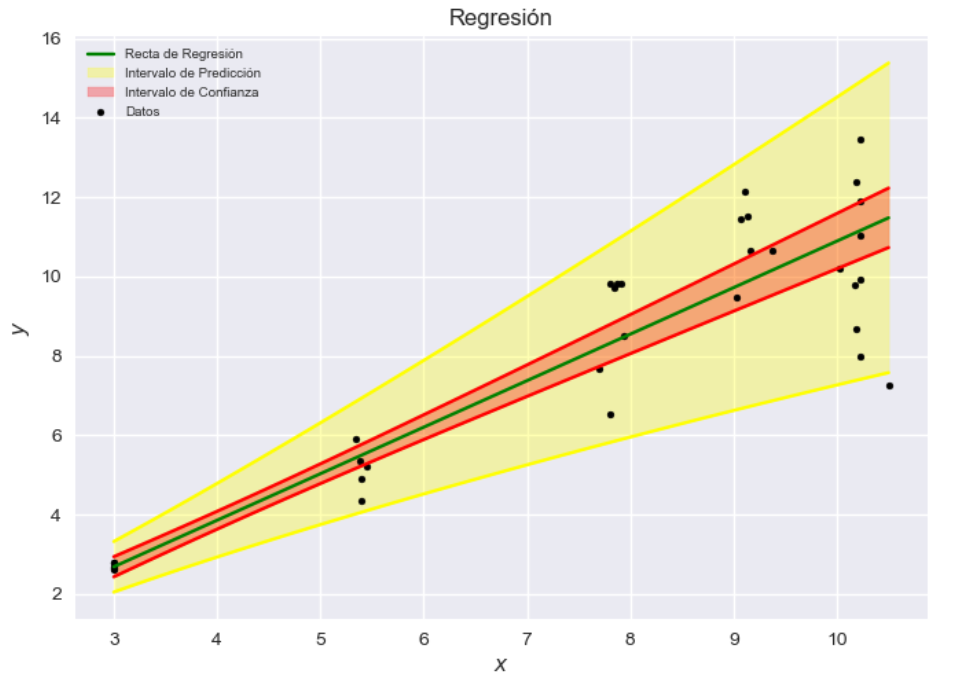
\includegraphics[scale=0.40]{Regresión MCP.png}
 \caption{Modelo de Regresión Lineal Simple Ajustado por MCP, con Bandas de Predicción y Confianza al \(95\%\).}
 \label{fig:17}
\end{figure}

Por otra parte observe la gráfica presentada en la Figura \ref{fig:18}, recuerde que para obtener las estimaciones para \(\beta\) \eqref{ponde}, el modelo \eqref{model2} debía ser transformado a un modelo cuyos términos de error fueran de media cero, varianza constante y correlación \(0\), por lo que se graficaron los residuales del modelo transformado contra los valores ajustados de \(Y\) para analizar si existía alguna mejoría en la dispersión de los mismos\footnote{Esperando que estos se comportaran como las estimaciones de términos de error de media cero y varianza constante.}, a través de los distintos valores ajustados, usando que los residuales en el modelo transformado quedan dados por: 
\[
f = K^{-1}e, 
\]
con \(e\) los residuales del modelo original y 
\[
K^{-1} = diag(\sqrt{\omega_1}, \hdots, \sqrt{\omega_{33}}),
\]
No es difícil observar que la dispersión de los residuales mejoró bastante, respecto a la presentada en la gráfica del inciso \textbf{(c)}. No se presenta una gráfica contra los valores de la variable independiente,\footnote{Aunque la misma puede consultarse en el script adjunto, para constatar lo que aquí se ha dicho.} debido a que nuevamente existe bajo el modelo de regresión lineal por MCP un coeficiente de pendiente positivo relativamente cercano a 1, y por ende, al igual que en los incisos \textbf{(b)} y \textbf{(c)} se obtendrían resultados similares. Por último, si se comparan los coeficientes de determinación del modelo de regresión lineal simple ajustado con MCP \eqref{R^222} contra el mismo coeficiente para el modelo de regresión lineal simple ajustado con MCO \eqref{R^21}, uno se percata que bajo el modelo ajustado con MCP la cantidad de variabilidad de la variable dependiente \(Y\), explicada por la variable independiente \(X\) es mayor. Por lo que, bajo estos tres criterios se concluye que el modelo de regresión lineal simple ajustado por MCP tiene un mejor ajuste a los datos proporcionados. 

\begin{figure}[htb]
 \centering
 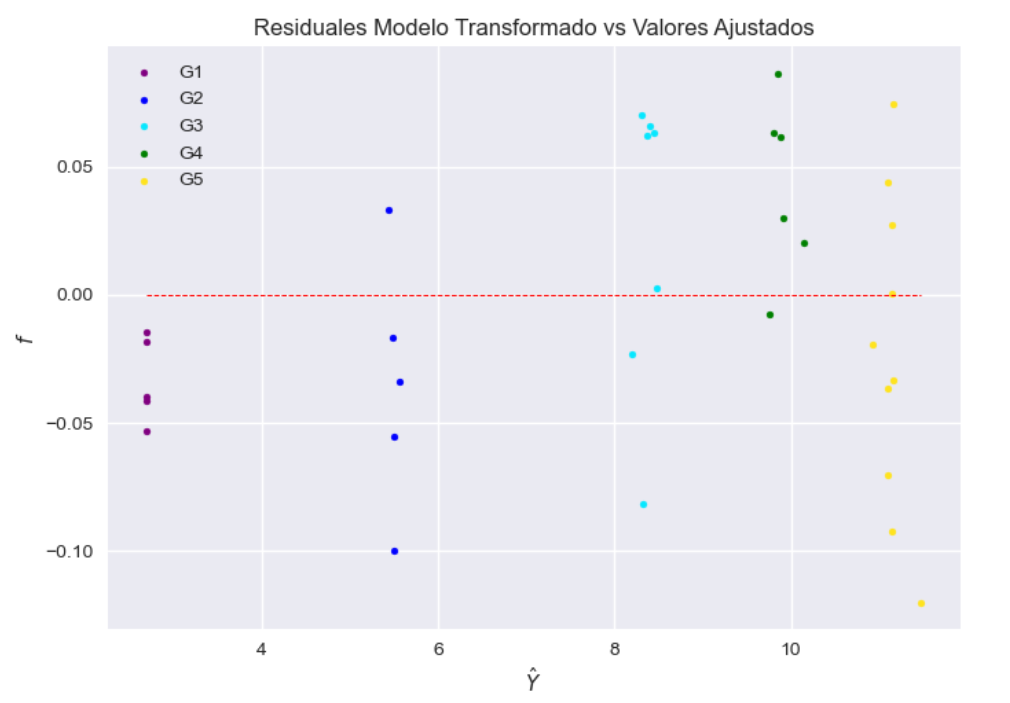
\includegraphics[scale=0.40]{Resid vs Ajustes.png}
 \caption{Residuales del Modelo Transformado vs Valores Ajustados para Y.}
 \label{fig:18}
\end{figure}

\end{solucion}

%%%%%%%%%%%%%%%%%%%%%%%%%%%%%%%%%%%%%%%%%%%%%%%%%%%%%%%%%%%%%%%%%%%%%%%%%%%%%%%%%%%%%%%%%%%%%%%%%%%%%%%%%%%%%%%%%%%%%%%%%%%%%%%%%%%%%%%%%%%%%%%%%%%%%%%5
\setcounter{exo}{1}
\begin{exo}
Considerando los datos que se muestran en la Figura \ref{fig:2}, donde se presentan veinte valores de 
las variables explicativas $X_0, X_1, X_2,$ $Z_1$ y $Z_2$, asi como de la variable respuesta $Y$, se pide reproducir las 
expresiones y hacer los cálculos que se indican en los cinco incisos del Teorema visto en la clase del 
miércoles. 


\begin{itemize}
\item[(a)] Con base en los datos de la Tabla 2, construya la matriz de diseño $X$ formada por las columnas $X_0, X_1$ y 
$X_2$, así como también la matriz $Z$ de regresores adicionales formada por las columnas $Z_1$ y $Z_2$. Además 
construya las matrices $W,R_G,L $ y$M$ , que se describen al inicio del Teorema. 
\item[(b)] Haga las cuentas matriciales y presente los resultados que se indican en los incisos (i), (ii), (iii), (iv) y 
(v). 
\end{itemize}
\end{exo}
\begin{solucion}
\begin{figure}[htb]
 \centering
 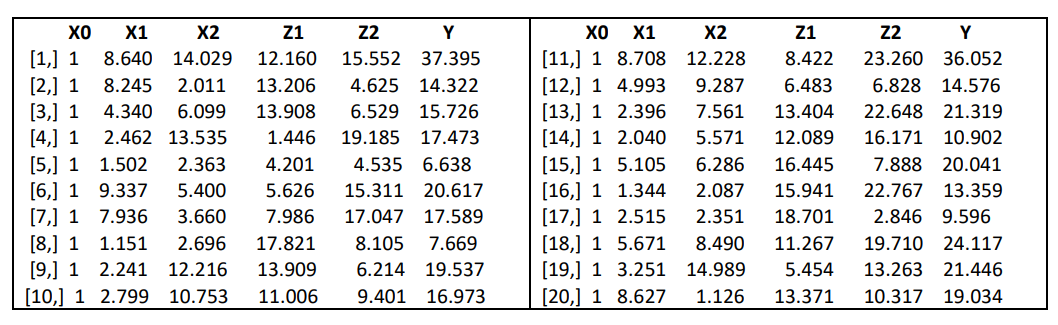
\includegraphics[scale=0.4]{T3T2.png}
 \caption{Valores de las variables explicativas \(X_0,X_1\) y \(X_2\), así como las covariables adicionales \(Z_1\),\(Z_2\) y de la covariable \(Y\).}
 \label{fig:2}
\end{figure}
\end{solucion}
\textbf{(a)} La matriz de diseño \(X\), la matriz de regresores adicionales \(Z\) y la matriz con los valores de la variable dependiente \(Y\) se presentan a continuación: 
\begin{equation}\label{2.1}
X=\begin{pmatrix}
1 &8.640 &14.029  \\ 
 1& 8.245 &2.011\\
 1& 4.340 &6.099\\
 1& 2.462 &13.535\\
 1& 1.502 &2.363 \\
 1& 9.337 &5.400 \\
 1& 7.936 &3.660 \\
 1& 1.151 &2.696\\
1& 2.241 &12.216\\
 1& 2.799 &10.753\\
 1 &8.708 &12.228 \\
1& 4.993 &9.287 \\
1& 2.396 &7.561 \\
1& 2.040 &5.571\\
1& 5.105& 6.286\\
1& 1.344& 2.087\\
1& 2.515& 2.351\\
 1& 5.671& 8.490\\
1 &3.251& 14.989\\
1 &8.627& 1.126   
\end{pmatrix},\quad Z=\begin{pmatrix}
12.160 &15.552\\
13.206 &4.625\\  
13.908 &6.529\\
1.446 &19.185\\
4.201 &4.535\\
5.626 &15.311\\
7.986 &17.047\\
17.821 &8.105\\
13.909 &6.214\\  
11.006 &9.401\\ 
8.422 &23.260\\
6.483 &6.828\\
13.404 &22.648\\
12.089 &16.171\\
16.445 &7.888\\
15.941 &22.767\\
18.701 &2.846\\
11.267 &19.710\\
5.454 &13.263\\
13.371 &10.317
\end{pmatrix} \quad 
Y = \begin{pmatrix}
 37.395\\
 14.322\\
 15.726\\
 17.473\\
  6.638\\
 20.617\\
 17.589\\
  7.669\\
 19.537\\
 16.973\\
 36.052\\
 14.576\\
 21.319\\
 10.902\\
 20.041\\
 13.359\\
  9.596\\
 24.117\\
 21.446\\
 19.034
\end{pmatrix},
\end{equation}
Ahora, se supondrá que se busca ajustar un modelo de la forma 
\begin{equation}\label{2.2}
    E[Y|X,Z] = \begin{pmatrix}
    X & Z
    \end{pmatrix}
    \begin{pmatrix}
    \beta_{G} \\
    \gamma_{G}
    \end{pmatrix} = W \delta_{G}, 
\end{equation}
y que uno de la forma 
\begin{equation}\label{2.3}
    E[Y|X] =  X \beta,
\end{equation}
fue ajustado con anterioridad obteniendo como estimación para \(\beta\) al siguiente vector 
\begin{equation}\label{2.4}
\hat{\beta}=(X^{'}X)^{-1}X^{'}Y \begin{pmatrix}
    2.722\\ 1.643\\ 1.097
    \end{pmatrix}.
\end{equation}
Utilizando las matrices en \eqref{2.1}, entonces es posible obtener las matrices \(W,L,M, R_{G},R\) comentadas\footnote{Los cálculos de las mismas fueron hechos con Julia, los resultados aquí se presentan redondeados a tres dígitos.} en el \textbf{Teorema \ref{Teoremita}} y quedan dadas de la siguiente manera: 
\begin{equation}\label{W}
    W = \begin{pmatrix}X , Z\end{pmatrix} = \begin{pmatrix}
1 &8.640 &14.029 &12.160 &15.552\\
 1& 8.245 &2.011&13.206 &4.625\\  
 1& 4.340 &6.099 & 13.908 &6.529\\
 1& 2.462 &13.535 & 1.446 &19.185\\
 1& 1.502 &2.363 &4.201 &4.535\\
 1& 9.337 &5.400 &5.626 &15.311\\
 1& 7.936 &3.660 &7.986 &17.047\\
 1& 1.151 &2.696 &17.821 &8.105\\
1& 2.241 &12.216 &13.909 &6.214\\ 
 1& 2.799 &10.753 &11.006 &9.401\\ 
 1 &8.708 &12.228 &8.422 &23.260\\
1& 4.993 &9.287 &6.483 &6.828\\
1& 2.396 &7.561 &13.404 &22.648\\
1& 2.040 &5.571& 12.089 &16.171\\
1& 5.105& 6.286 & 16.445 &7.888\\
1& 1.344& 2.087 &15.941 &22.767\\
1& 2.515& 2.351&18.701 &2.846\\
 1& 5.671& 8.490 &11.267 &19.710\\
1 &3.251& 14.989 &5.454 &13.263\\
1 &8.627& 1.126 &13.371 &10.317  
\end{pmatrix},
\end{equation}
\begin{equation}\label{L,M}
    L = (X^{'}X)^{-1}X^{'}Z =\begin{pmatrix}
15.587& 8.074\\
-0.267& 0.309\\
-0.448& 0.433\\
\end{pmatrix} ,\quad M = (Z^{'}R Z)^{-1} = \begin{pmatrix}
3.009\cdot 10^{-3} &2.253\cdot 10^{-4}\\
2.253\cdot 10^{-4} &1.328\cdot 10^{-3} 
\end{pmatrix}.
\end{equation}
Dado que las matrices \(R_G\) y \(R\) son de tamaño \(20\times20\) pueden ser consultadas en el script adjunto a esta tarea por cuestiones de espacio.\\

\textbf{(b)} Para corroborar los incisos \((i)\) y \((ii)\) del \textbf{Teorema \ref{Teoremita}}, primero se realizo un calculo directo del estimador de MCO para el vector de parámetros \(\delta\) del modelo \eqref{2.2} utilizando la matriz \(W\) \eqref{W} lo que dio como resultado
\begin{equation}\label{deltadir}
    \hat{\delta}_{G} =(W^{'}W)^{-1}W^{'}Y = \begin{pmatrix} -8.495\\1.672\\ 1.177\\ 0.531\\ 0.365 \end{pmatrix},
\end{equation}
luego se calculo por separado \(\hat{\beta}_G\) y \(\hat{\gamma}_{G}\) de acuerdo a los incisos \((i)\) y \((ii)\)\footnote{En el script adjunto se calcularon los rangos de \(X\) y \(Z\) con el fin de verificar que ambas fueran de rango completo, y el rango de \(W\) para confirmar que las columnas de \(X\) y \(Z\) fueran \(l.i\).} del \textbf{Teorema \ref{Teoremita}}, es decir que 
\begin{equation}\label{gamma}
    \hat{\gamma}_{G} = (Z^{'}R Z)^{-1}Z^{'}RY= MZ^{'}RY = \begin{pmatrix}0.531\\ 0.365 \end{pmatrix}.
\end{equation}
Posteriormente se calculo de las dos formas indicadas en el inciso \((i)\) el valor de \(\hat{\beta}_{G}\), es decir 
\begin{equation}\label{forma1}
    \hat{\beta}_{G} = (X^{'}X)^{-1}X^{'}(Y - Z \hat{\gamma}_{G}) = \begin{pmatrix}-8.495\\ 1.672\\ 1.177 \end{pmatrix},
\end{equation}
y usando \(\hat{\beta}\) en \eqref{2.4}, es decir
\begin{equation}\label{forma2}
   \hat{\beta}_{G} =  \hat{\beta} - L \hat{\gamma}_{G} = \begin{pmatrix}-8.495\\ 1.672\\ 1.177 \end{pmatrix},
\end{equation}
de \eqref{forma1} y \eqref{forma2} se observa que ambos cálculos para \(\hat{\beta}_{G}\), son iguales bajo redondeo a tres dígitos, como era de esperarse. Luego de \eqref{gamma}, \eqref{forma1} y \eqref{forma2} se tiene que 
\begin{equation}\label{deltanodir}
    \begin{pmatrix}\hat{\beta}_{G} \\ \hat{\gamma}_{G} \end{pmatrix} =  \begin{pmatrix} -8.495\\1.672\\ 1.177\\ 0.531\\ 0.365 \end{pmatrix}.
\end{equation}
Comparando \eqref{deltadir} y \eqref{deltanodir}, se confirman los incisos \((i)\) y \((ii)\) bajo redondeo a 3 dígitos. 
%%%%%%%%%%%%%%%%%%%%%%%%%%%%%%%%%%%%%%%%%%%%%%%%%%%%%%%%%%%%%%%%%%%%%%%%%%%%%%%%%%%%%%%%%%%%%%%%%%%%%%%%%%%%%%%%%%%%%%%%%%%%%%%%%%%%%%%%%%%%%%%%%%%%%%
Para corroborar los incisos \((iii)\) y \((iv)\), bastará observar que 
\begin{equation}\label{forma11}
    Y^{'}R_{G}Y = 84.892, 
\end{equation}
donde como ya se comento con anterioridad la matriz \(R_G\) puede consultarse en el script adjunto. Luego
\begin{equation}\label{forma12}
    (Y - Z \hat{\gamma}_{G})^{'}R(Y - Z \hat{\gamma}_{G}) = 84.892, 
\end{equation}
donde \(Y,Z\) están dados en \eqref{2.1}, la matriz \(R\) puede consultarse en el script adjunto y \(\gamma_{G}\) como en \eqref{gamma}. Por último
\begin{equation}\label{forma13}
     Y^{'}RY - \hat{\gamma}_{G}^{'}Z^{'}RY = 84.892. 
\end{equation}
Los resultados \eqref{forma11}, \eqref{forma12} y \eqref{forma13} corroboran los inciso \((iii)\) y \((iv)\) bajo redondeo a tres dígitos. Por último, para el inciso \((v)\) se llevo a cabo un cálculo directo de la matriz de covarianzas de \(\hat{\delta}_{G}\) de la siguiente forma 
\begin{equation}\label{covas1}
    cov(\hat{\delta}_{G}) = \sigma^2(W^{'}W)^{-1} = 
\sigma^2\begin{pmatrix}
  1.1835 & -0.0370 &  -0.0334 &  -0.0487 &  -0.0142\\
 -0.0370 &  0.0065 &   0.0004 &   0.0007 &  -0.0004\\
 -0.0334 &  0.0004 &   0.0033 &   0.0013 &  -0.0005\\
 -0.0487 &  0.0007 &   0.0013 &   0.0030 &   0.0002\\
 -0.0142 & -0.0004 &  -0.0005 &   0.0002 &   0.0013
\end{pmatrix},
\end{equation}
Luego utilizando el \textbf{Teorema \ref{Teoremita}} se obtuvo lo siguiente: \footnote{Los redondeos aquí fueron a cuatro decimales porque con menos dígitos algunas cifras se anulaban.}
\begin{equation}\label{Yaacabamierda}
    (X^{'}X)^{-1} + LML^{-1} = \begin{pmatrix}
  1.1835&  -0.0370& -0.0334\\
 -0.0370&   0.0065&  0.0004\\
 -0.0334&   0.0004&  0.0033
\end{pmatrix}\end{equation}
\begin{equation}\label{Yaacabamierda1}
 -LM = \begin{pmatrix}
 -0.0487&  -0.0142\\
  0.0007&  -0.0004\\
  0.0013&  -0.0005
    \end{pmatrix},\quad -ML^{'} = (-LM)^{'}. 
\end{equation}
Y la matriz \(M\), redondeada a 4 dígitos esta dada por:
\begin{equation}\label{MMM}
M = \begin{pmatrix}
 0.0030&  0.0002\\ 
 0.0002&  0.0013
\end{pmatrix},  
\end{equation}
de este modo se sigue de \eqref{Yaacabamierda}, \eqref{Yaacabamierda1} y de \eqref{MMM} que
\begin{align}\label{covas2}
    cov(\hat{\delta}_{G})&=\sigma^2\begin{pmatrix}(X^{'}X)^{-1} + LML^{-1}&-LM\\ -ML^{'} & M \end{pmatrix}\nonumber\\
    &= \sigma^2\begin{pmatrix}
  1.1835&  -0.0370 &  -0.0334&  -0.0487&  -0.0142\\
 -0.0370&    0.0065&   0.0004&   0.0007&  -0.0004\\
 -0.0334&   0.0004&   0.0033&   0.0013&  -0.0005\\
 -0.0487&   0.0007&   0.0013&   0.0030&    0.0002\\
 -0.0142&  -0.0004&  -0.0005&   0.0002&   0.0013
\end{pmatrix},
\end{align}
Entonces por \eqref{covas1} y \eqref{covas2} se sigue la igualdad establecida, redondeando a 4 dígitos.


\section{Anexo}
\textbf{A.Ejercicio 1.}
El \(R^2\) en un modelo de regresión lineal múltiple con matriz de diseño \(X\) y respuesta \(Y\) que no considera intercepto esta dado por: 
\[
R^2 = \frac{\hat{Y}^{'}\hat{Y}}{Y^{'}Y}.
\]

\textbf{A.Ejercicio 2.}
\begin{thm}\label{Teoremita}
Sea \(X\) matriz de \(n x p\) tal que \(p < n\) de rango \(p\), y sea \(Y\) un vector de \(n\times 1\), suponga que un modelo
\begin{equation}\label{A.1}
    E[Y|X] =  X \beta,
\end{equation}
fue ajustado por mínimos cuadrados ordinarios con anterioridad, dando como estimación para el vector \(\beta\) a \(\hat{\beta}\). Y suponga que \(Z\) es una matriz de covariables adicionales de \(n \times t\) con rango \(t <n\) y tal que \(t + p < n\), las cuales se quieren añadir al modelo, entonces si las columnas de \(Z\) son l.i de las columnas de \(X\) se cumplirá para el modelo
\begin{equation}\label{A.2}
    E[Y|X,Z] = \begin{pmatrix}
    X, Z
    \end{pmatrix}
    \begin{pmatrix}
    \beta_{G}, \\
    \gamma_{G}
    \end{pmatrix} = W \delta_{G}, 
\end{equation}
que si se definen \(L = (X^{'}X)^{-1}X^{'}Z\), \(R = I_{n\times n} - X(X^{'}X)X^{'}\), \(R_{G} = I_{n\times n} - W(W^{'}W)W^{'}\), \(M = (Z^{'}R Z)^{-1}\), y \(\hat{\delta}_{G} = \begin{pmatrix}\hat{\beta}_{G}\\ \hat{\gamma}_{G}\end{pmatrix}\) denota al estimador de MCO para el modelo \eqref{A.2} entonces:
\begin{itemize}
    \item[(i)] \(\hat{\beta}_{G} = (X^{'}X)^{-1}X^{'}(Y - Z \hat{\gamma}_{G}) = \hat{\beta} - L \hat{\gamma}_{G}.\) 
    \item[(ii)] \(\hat{\gamma}_{G} = (Z^{'}R Z)^{-1}Z^{'}RY= MZ^{'}RY.\)
    \item[(iii)] \(Y^{'}R_{G}Y = (Y - Z \hat{\gamma}_{G})^{'}R(Y - Z \hat{\gamma}_{G}).\)
    \item[(iv)] \(Y^{'}R_{G}Y = Y^{'}RY - \hat{\gamma}_{G}^{'}Z^{'}RY.\)
    \item[(v)] \(V(\hat{\delta}_{G}) = \sigma^2\begin{pmatrix}(X^{'}X)^{-1} + LML^{-1}&-LM\\ -ML^{'} & M \end{pmatrix}.\)
\end{itemize}
\end{thm}



\end{document}
